\documentclass[boxes]{gsypset}

% Info for header
\mailbox{}
\initials{}
\collaborators{}
\class{Math 65}
\assignment{HW 11}
\duedate{June 1, 2016}

\usepackage{hyperref}

\begin{document}
	\begin{problem}
		Consider the planar autonomous system 
		\begin{align*}
			x'(t) &= 1-y^2\\
			y'(t) &= 1-x^2
		\end{align*}
		
		\begin{subproblems}
			\subproblem 
				What are the $x$- and $y$-nullclines of the DEs? 
				Use these nullclines to determine the regions of the plane in which 
				the solution orbits would be moving left, right, up, and down.
				\begin{solution}
					
				\end{solution}
			\subproblem 
				Locate all the equilibrium points of the system 
				by finding the intersections of the nullclines.
				\begin{solution}
					
				\end{solution}
			\subproblem 
				Print out a phase plane portrait of the DE in the rectangle $|x|\leq 3, |y| \leq 3$ 
				using either pplane\footnote{\url{http://math.rice.edu/~dfield/dfpp.html}} or
				ODEToolkit\footnote{\url{http://odetoolkit.hmc.edu}}. 
				Explain how this phase plane portrait is consistent with all of the 
				observations you've made on this problem.
				\begin{solution}
					
				\end{solution}
			\subproblem 
				For each equilibrium point you found in part (b), 
				(i) write down the linearized differential equation about that point, 
				(ii) calculate the eigenvalues of the linearized system, 
				(iii) use the eigenvalues to determine the behavior (unstable/stable, node/spiral, etc.) 
				of the linearized system near each point.
				\begin{solution}
					
				\end{solution}
		\end{subproblems}
	\end{problem}
	
	\begin{problem}
		Here's a phase plane portrait for a planar, autonomous system of DEs.
		Find a system of DEs that matches this phase plane portrait as best as you can. 
		Use software to print out your phase plane portrait. 
		Explain thoroughly (using nullclines, where the solutions are moving left/right/up/down, 
		equilibrium points) why your system of DEs matches the given phase plane portrait.
		\begin{center}
			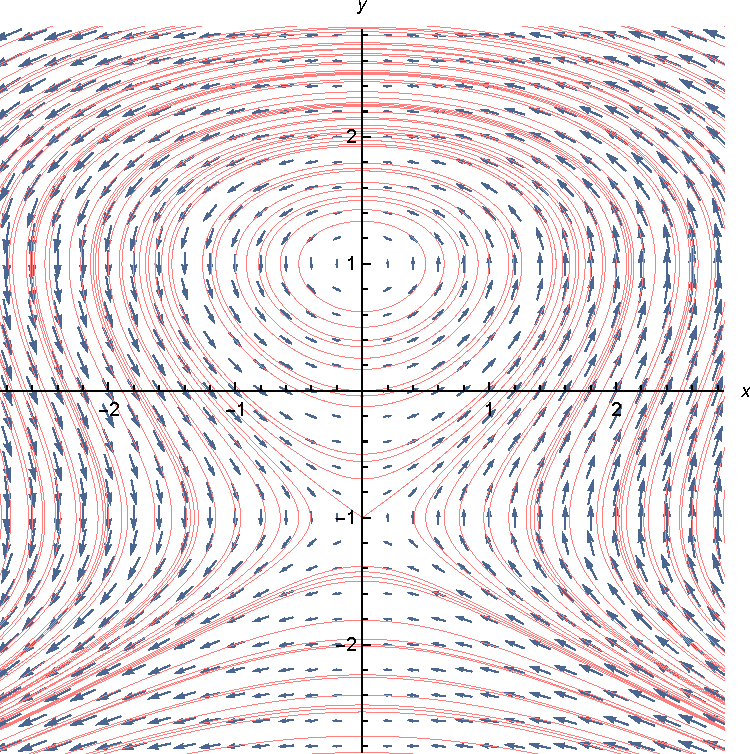
\includegraphics[height=3.7in,keepaspectratio=true]{img/hw11-02}
		\end{center}
	\end{problem}
	\begin{solution}
		
	\end{solution}
	
	\begin{problem}
		Consider the linear, constant-coefficient, homogeneous differential equation system
		\[
			\mathbf{x}'(t) = \bm{x'(t) \\ y'(t)} = \bm{a & b \\ c & d}\bm{x(t) \\ y(t)}.
		\]
		Pick values of $a$, $b$, $c$, and $d$ so that the equilibrium point at the origin is 
		\begin{itemize}
			\item an unstable saddle point,
			\item an improper node (asymptotically stable or unstable, your choice),
			\item a center (neutrally stable), and
			\item a spiral (asymptotically stable or unstable, your choice).
		\end{itemize}
		Use software to print out a phase plane portrait for each case. 
		On top of your portrait, plot the nullclines and show that 
		solution curves cross them in the proper way.
	\end{problem}
	\begin{solution}
		
	\end{solution}
	
	\begin{problem}
		A $m$~kg mass is suspended at the end of a (massless) rod with length $L$~meters. 
		The other end of the rod is fixed at a pivot point. 
		This arrangement that leads to a simple pendulum that swings in a plane. 
		Let $\theta(t)$ be the angular position of the pendulum, measured so that 
		the resting position of the pendulum corresponds to $\theta=0$ and 
		positive $\theta$ is in the direction of the arrow below.
		
		\begin{center}
			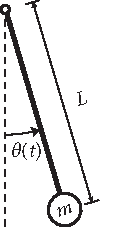
\includegraphics[width=.75in,keepaspectratio=true]{img/pendulum}
		\end{center}
		
		There are two forces acting on the pendulum: gravity and friction. 
		You may assume that the friction (due to air resistance or friction in the pivot) 
		causes a torque that is proportional to the angular velocity, $\dot{\theta}$.
		 
		\begin{subproblems}
			\subproblem 
				First, derive a governing equation using the rotational analog of Newton's second law, 
				$\tau=I\ddot{\theta}$. 
				(See Chapter 18 of your Physics 24 textbook.) 
				You can assume that the mass is concentrated at a point and the rod is massless, 
				so the moment of inertia of the mass is $I=mL^2$.  
				You should obtain the differential equation
				\[
					\ddot{\theta} + c\dot{\theta} + \frac{g}{L}\sin\theta = 0.
				\]
				What must be the units of the damping constant $c$?
				\begin{solution}
					
				\end{solution}
			\subproblem 
				Write your second-order differential equation as a system of first-order equations 
				by defining $\omega(t)=\dot{\theta}(t)$. 
				Are they linear or nonlinear? 
				Autonomous or nonautonomous?
				\begin{solution}
					
				\end{solution}
			\subproblem 
				Locate the equilibrium points of this system. 
				(There are infinitely many of them.) 
				What physical arrangement of the pendulum corresponds to each equilibrium point?
				\begin{solution}
					
				\end{solution}
			\subproblem 
				Use software to sketch phase plane portraits for two cases: 
				zero damping and some positive damping. 
				(You will need to pick some reasonable values for your parameters.) 
				Draw nullclines on top of your phase plane portraits and 
				verify that the solution curves pass through them in the proper way.
				\begin{solution}
					
				\end{solution}
		\end{subproblems}
	\end{problem}
	
	\begin{problem}
		In class, we considered the competitive species population model.
		\begin{align*}
			x'(t) &= x(r_1-a_1x-b_1y) \\
			y'(t) &= y(r_2-a_2y-b_2x)
		\end{align*} 
		All of the parameters in the DE above ($r_1$, $a_1$, $b_1$, $r_2$, $a_2$, $b_2$) are positive, 
		and we restrict our attention to $x\geq 0$ and $y\geq 0$ only. 
		Depending on these four constants, 
		there were four different (nondegerate) cases to be considered:
		\begin{itemize}
			\item 
				In case 1, the $x$-nullcline (blue) is completely below the
			  $y$-nullcline in the first quadrant and the species represented by
			  $x$ always goes extinct for any positive initial population values.
			\item 
				In case 2, the $y$-nullcline (red) is completely below the $x$-nullcline 
				in the first quadrant and the species represented by $y$ 
				always goes extinct for any positive initial population values.
			\item 
				In case 3, the two nullclines intersect at a point in the first quadrant. 
				That point is a stable equilibrium point. 
				The two populations always tend to a state where both populations coexist.
			\item 
				In case 4, the two nullclines intersect at a point in the first quadrant. 
				That point is an unstable saddle point. 
				One population will always go extinct but 
				which population goes extinct depends on the initial condition.
		\end{itemize}
		\hmcbreakproblem
		In this problem, you will complete the local stability analysis of this system of DEs.
		\begin{subproblems}
			\subproblem 
				In all four cases, there are at least two other equilibrium points: 
				one in which the $x$-population goes extinct but the other doesn't, and 
				one in which the $y$-population goes extinct but the other doesn't.  
				Calculate the locations of these two equilibrium points.
				\begin{solution}
					
				\end{solution}
			\subproblem 
				Sketch the nullclines for case 1 and locate the $x$- and $y$-intercepts of both nullclines.  
				What two inequalities must hold true for the $x$-nullcline to be 
				completely below the $y$-nullcline in the first quadrant?  
				Calculate the eigenvalues of $D\mathbf{f}(\mathbf{x}_{\text{eq}})$ 
				for both equilibrium points you found in part (b). 
				What do these eigenvalues tell you about the stability of the linearized system 
				near these equilibrium points?
				\begin{solution}
					
				\end{solution}
			\subproblem Repeat part (b) for case 2.
				\begin{solution}
					
				\end{solution}
			\subproblem 
				Determine the pairs of inequalities that must hold true to get cases 3 and 4. 
				(Refer to the lecture notes to see how the nullclines intersect each other.)
				\begin{solution}
					
				\end{solution}
			\subproblem 
				Consider the parameter values $r_1=a_1=b_1=a_2=1$, $r_2=1/2$, and $b_2=1/4$. 
				According to your work from part (d), 
				which case does this set of parameter values fall under? 
				Locate the equilibrium point for which $x>0$ and $y>0$. 
				Calculate the eigenvalues of $D\mathbf{f}(\mathbf{x}_{\text{eq}})$ for this equilibrium point 
				to determine the behavior of solutions near it. 
				(It is easier to use the parameter values that are given 
				rather than perform the calculation for a general set of parameter values.)
				\begin{solution}
					
				\end{solution}
			\subproblem 
				Locate the equilibrium point where both populations coexist 
				(whether the equilibrium point is stable or not) in cases 3 and 4. 
				Your answer will involve $r_1$, $a_1$, $b_1$, $r_2$, $a_2$, and $b_2$.
				\begin{solution}
					
				\end{solution}
		\end{subproblems}
	\end{problem}
\end{document}

